%%%%%%%%%%%%%%%%%%%%%%%%%%%%%%%%%%%%%%%%%%%%%%%%%%%%%%%%%%%%%%%%%%%%%%%%
%%%  THIS TEX FILE IS TO GENERATE PDF FILE FOR 
%%%     DATA MINING HOMEWORK 02
%%%  COPYRIGHT (C) JIMMY LIN, 2013, UT AUSTIN
%%%%%%%%%%%%%%%%%%%%%%%%%%%%%%%%%%%%%%%%%%%%%%%%%%%%%%%%%%%%%%%%%%%%%%%%
\documentclass[11pt,a4paper]{article}
%%%%%%%%%%%%%%%%%%%%%%%%%%%%%%%%%%%%%%%%%%%%%%%%%%%%%%%%%%%%%%%%%%%%%%%%
%%%  PACKAGES USED IN THIS TEX SOURCE FILE
%%%%%%%%%%%%%%%%%%%%%%%%%%%%%%%%%%%%%%%%%%%%%%%%%%%%%%%%%%%%%%%%%%%%%%%%
\usepackage{geometry,amsthm,amsmath,graphicx,fancyheadings,framed}
\usepackage{tikz}
\usepackage{fancybox}
\usepackage[]{./mcode}
\usetikzlibrary{automata,positioning}
\usepackage[colorlinks,
            linkcolor=blue,
            anchorcolor=red,
            citecolor=green
            ]{hyperref}
\usepackage{/Users/JimmyLin/workspace/latexTemplate/UTA_CS/JS}
\usepackage{/Users/JimmyLin/workspace/latexTemplate/UTA_CS/JSASGN}
%%%%%%%%%%%%%%%%%%%%%%%%%%%%%%%%%%%%%%%%%%%%%%%%%%%%%%%%%%%%%%%%%%%%%%%%
%%% MACROS CONTAINING THE FILE INFORMATION
%%%%%%%%%%%%%%%%%%%%%%%%%%%%%%%%%%%%%%%%%%%%%%%%%%%%%%%%%%%%%%%%%%%%%%%%
\renewcommand{\COURSE}{CS363D Statistical Learning and Data Mining}
\renewcommand{\LECTURER}{Pradeep Ravikumar}
\renewcommand{\TUTOR}{Adarsh Prasad}
\renewcommand{\TASK}{Homework 02}
\renewcommand{\RELEASEDATE}{Feb. 25 2014}
\renewcommand{\DUEDATE}{Mar. 03 2014}
\renewcommand{\TIMECONSUME}{7 hours}
%%%%%%%%%%%%%%%%%%%%%%%%%%%%%%%%%%%%%%%%%%%%%%%%%%%%%%%%%%%%%%%%%%%%%%%%
%%% DOCUMENTATION STARTS FROM HERE 
%%%%%%%%%%%%%%%%%%%%%%%%%%%%%%%%%%%%%%%%%%%%%%%%%%%%%%%%%%%%%%%%%%%%%%%%
\begin{document}
%%%%%%%%%%%%%%%%%%%%%%%%%%%%%%%%%%%%%%%%%%%%%%%%%%%%%%%%%%%%%%%%%%%%%%%%
%% TITLE PAGE
%%%%%%%%%%%%%%%%%%%%%%%%%%%%%%%%%%%%%%%%%%%%%%%%%%%%%%%%%%%%%%%%%%%%%%%%
\begin{titlepage}
    \maketitle
\end{titlepage}
%%%%%%%%%%%%%%%%%%%%%%%%%%%%%%%%%%%%%%%%%%%%%%%%%%%%%%%%%%%%%%%%%%%%%%%%
%% CONTENT PAGE: TABLEOFCONTENTS, LISTOFTABLES, LIST OF FIGURES
%%%%%%%%%%%%%%%%%%%%%%%%%%%%%%%%%%%%%%%%%%%%%%%%%%%%%%%%%%%%%%%%%%%%%%%%
\renewcommand{\contentsname}{Contents}
\begin{center} 
    \tableofcontents 
    %\listoftables 
    \listoffigures
\end{center}
\newpage
%%%%%%%%%%%%%%%%%%%%%%%%%%%%%%%%%%%%%%%%%%%%%%%%%%%%%%%%%%%%%%%%%%%%%%%%
%%% GENERAL DOCUMENTATION BEGINS 
%%%%%%%%%%%%%%%%%%%%%%%%%%%%%%%%%%%%%%%%%%%%%%%%%%%%%%%%%%%%%%%%%%%%%%%%

\section{Data Transformation and Normalization}
\subsection{Transformation}
\begin{figure}[h]
    \centering
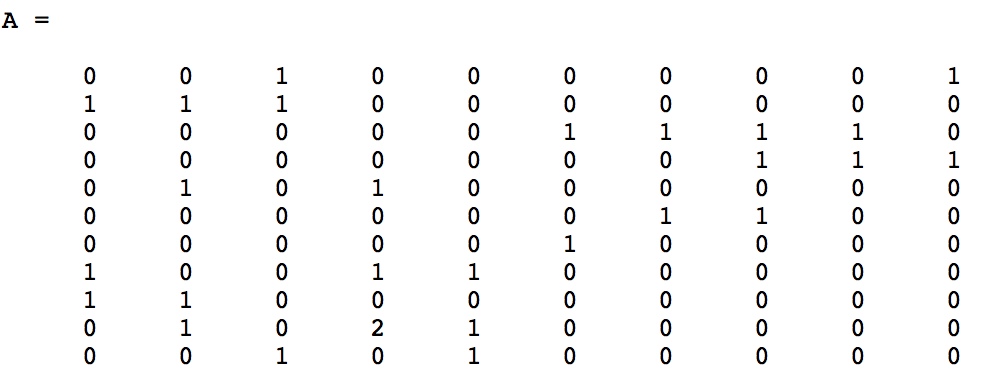
\includegraphics[width=4in,height=2.5in]{./A.png} \\
\end{figure}

where each document vector (column) correponds to the frequency of terms 
$$ (business, computer, economy, growth, operating, recession, recovery,
released, software, system, virus) $$
and each term vector (row) represents term frequency in documents
$$ 
(c1, c2, c3, c4, c5, m6, m7, m8, m9, m10)
$$

\subsection{Normalization}
\begin{figure}[h]
    \centering
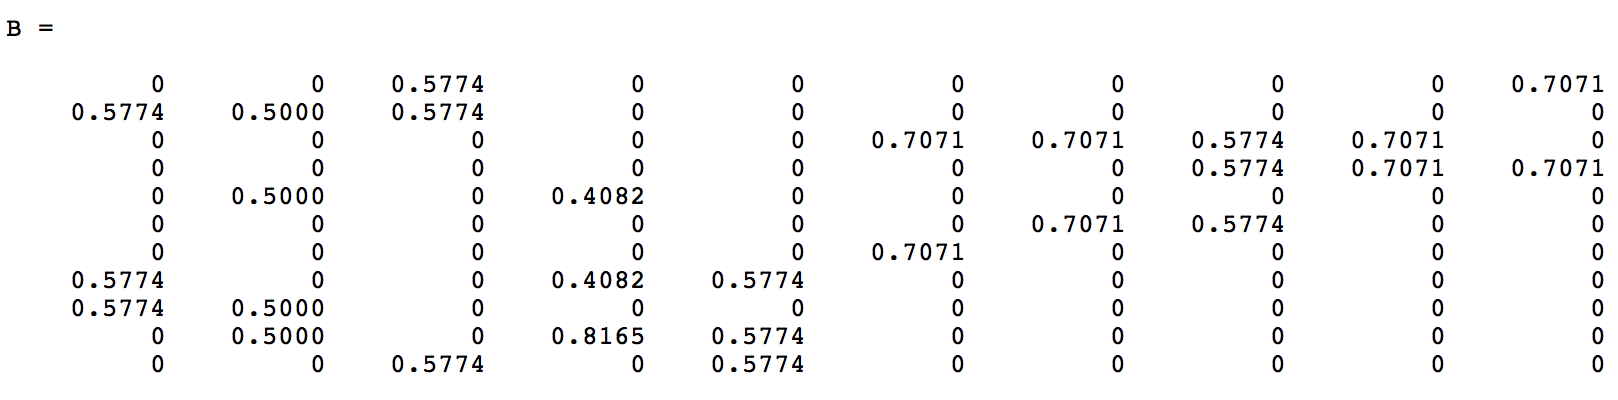
\includegraphics[width=6.5in,height=3in]{./B.png} \\
\end{figure}
\newpage

\section{Cosine Similarity}
We compute the $B^T B$ and get the following result,

\begin{figure}[h]
    \centering
    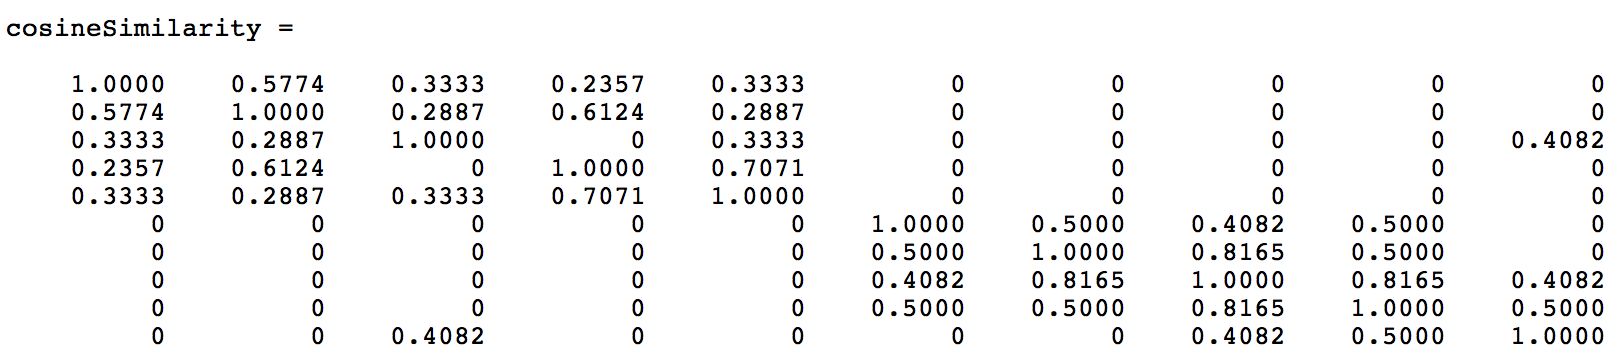
\includegraphics[width=6.5in,height=3.in]{./cosine.png} \\
\end{figure}

Note that each entry $e_{ij}$ represents the cosine similarity between
document $i$ and document $j$.
\newpage

\section{Singular Value Decomposition}
\begin{figure}[h]
    \centering
    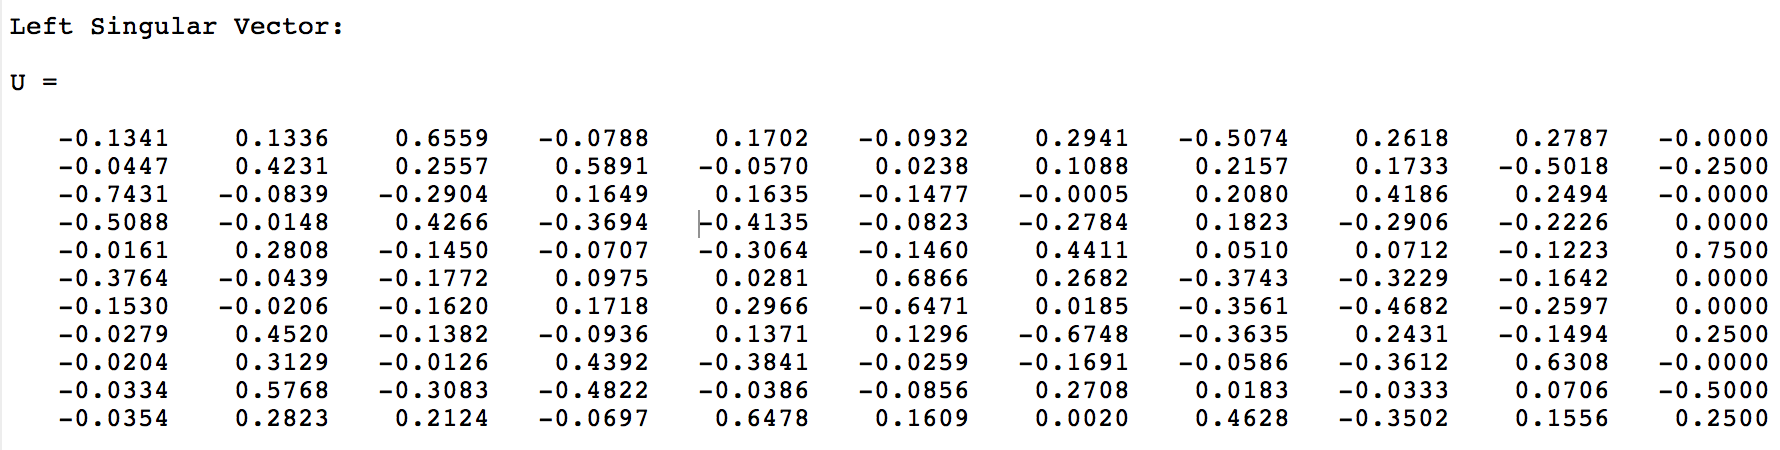
\includegraphics[width=6.5in,height=3.in]{./lsv.png} \\
    \caption{Each Column is a Left Singular Vector}
\end{figure}

\begin{figure}[h]
    \centering
    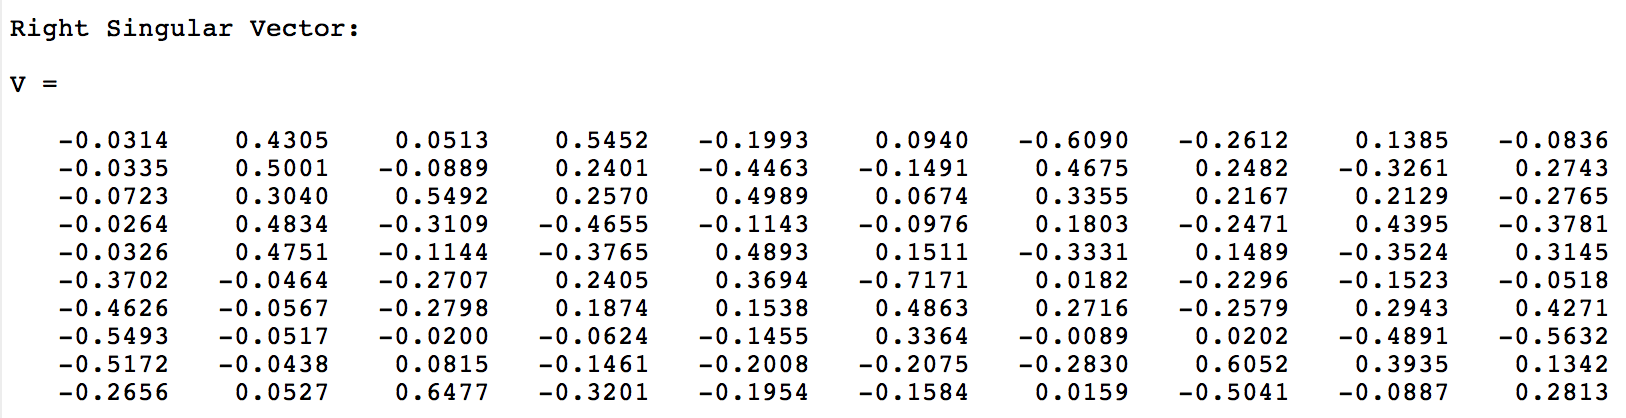
\includegraphics[width=6.5in,height=3.in]{./rsv.png} \\
    \caption{Each Column is a Right Singular Vector}
\end{figure}
   
Singluar Values are respectively, \\ 

    1.7114 ,   1.5933  ,  1.1817 ,   0.9899 ,   0.8807  ,  0.7837  ,  0.6969
    ,0.4560  ,  0.2300 ,   0.1409

\newpage
\section{Plot first two left/right singular matrix}

Two Left singular Vectors: \\
U1 = 
(-0.1341 ,  -0.0447 ,  -0.7431,   -0.5088  , -0.0161 ,  -0.3764  , -0.1530 ,
-0.0279  , -0.0204   -0.0334   -0.0354) \\
U2 =
(0.1336 ,   0.4231 ,  -0.0839 ,  -0.0148  ,  0.2808  , -0.0439  , -0.0206 ,
0.4520 ,   0.3129  ,  0.5768  ,  0.2823) \\[0.3cm]
Two Right singular Vectors: \\
V1 = 
(-0.0314 ,  -0.0335  , -0.0723 ,  -0.0264  , -0.0326 ,  -0.3702 ,  -0.4626,
-0.5493  , -0.5172  , -0.2656 )\\
V2 = 
    (0.4305  ,  0.5001 ,   0.3040  ,  0.4834   , 0.4751  , -0.0464 ,  -0.0567,
    -0.0517  , -0.0438  ,  0.0527 )\\

\begin{figure}[h]
    \centering
    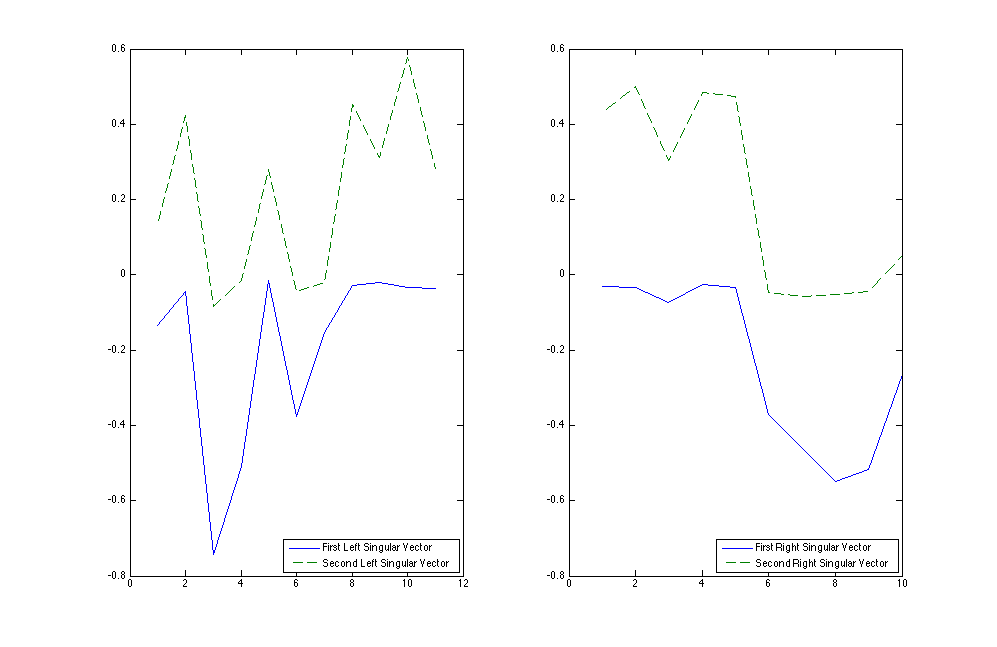
\includegraphics[width=7in,height=3.5in]{./4s.png} \\
    \caption{Two Left Columns and Right Columns}
\end{figure}

\newpage

\section{Plot the projected document vectors}
\begin{figure}[h]
    \centering
    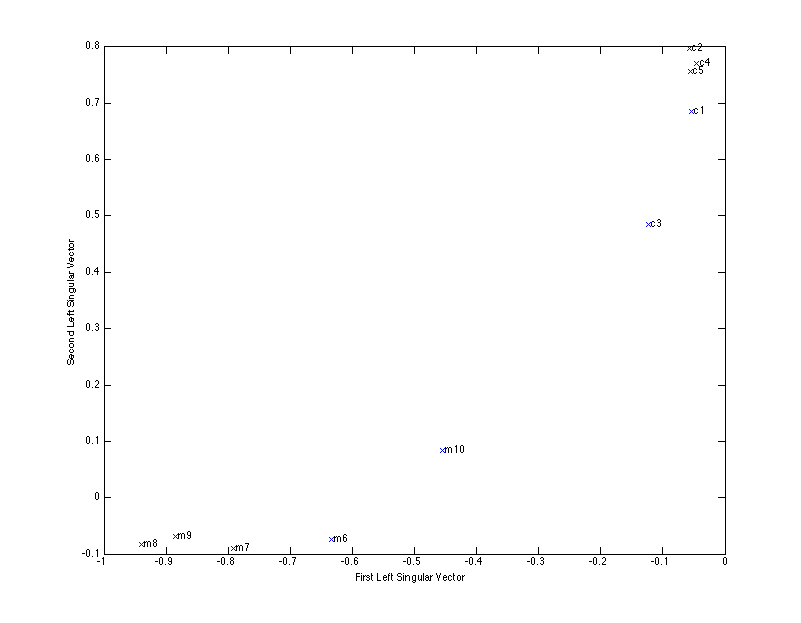
\includegraphics[width=7in,height=3.5in]{./5s.png} \\
    \caption{Projected Document Vectors}
\end{figure}

\section{Plot the projected term vectors}
\begin{figure}[h]
    \centering
    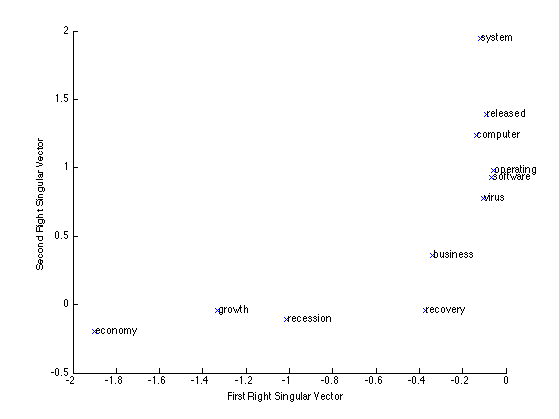
\includegraphics[width=7in,height=3.5in]{./6s.png} \\
    \caption{Projected Term Vectors}
\end{figure}

\newpage
\section{Source Code}
\lstinputlisting{./homework2.m}

%%%%%%%%%%%%%%%%%%%%%%%%%%%%%%%%%%%%%%%%%%%%%%%%%%%%%%%%%%%%%%%%%%%%%%%%
%%% General Documentation ends
%%%%%%%%%%%%%%%%%%%%%%%%%%%%%%%%%%%%%%%%%%%%%%%%%%%%%%%%%%%%%%%%%%%%%%%%
\end{document}
